\documentclass[12pt,twoside,a4paper]{report}
\usepackage[deti,newlogo]{uathesis}

% optional packages
\usepackage[portuguese]{babel}
\usepackage{hyperref}
\usepackage{amsmath}
\usepackage{amssymb}
\usepackage{xspace}
\usepackage{lipsum}
\usepackage{microtype}
\usepackage{multicol}
\usepackage{dirtytalk}
\usepackage{todonotes}
\usepackage[acronym,nonumberlist, nopostdot]{glossaries}
\newglossary[tlg]{nomenclature}{tld}{tdn}{Nomenclature}

\def\ThesisYear{2019}

% depth of the table of contents
\setcounter{tocdepth}{2}

% horizontal line to separate floats (figures and tables) from text
\def\topfigrule{\kern 7.8pt \hrule width\textwidth\kern -8.2pt\relax}
\def\dblfigrule{\kern 7.8pt \hrule width\textwidth\kern -8.2pt\relax}
\def\botfigrule{\kern -7.8pt \hrule width\textwidth\kern 8.2pt\relax}

\def\AddVMargin#1{\setbox0=\hbox{#1}
                  \dimen0=\ht0\advance\dimen0 by 2pt\ht0=\dimen0
                  \dimen0=\dp0\advance\dimen0 by 2pt\dp0=\dimen0
                  \box0}
\def\Header#1#2{\setbox1=\hbox{#1}\setbox2=\hbox{#2}
           \ifdim\wd1>\wd2\dimen0=\wd1\else\dimen0=\wd2\fi
           \AddVMargin{\parbox{\dimen0}{\centering #1\\#2}}}

\makenoidxglossaries
\loadglsentries{./src/glossary}

\begin{document}

% Cover pages and basic template importation requirements
% Cover pages and basic template importation requirements
% Change with your info -------------------------------------------------

\def\theauthor{Diogo Vala \newline Correia}
\def\thesistitle{Something about Smart Shelfs, UHF RFID and Item tagging}
\def\course{Master in Electronics and Telecommunications Engineering}

\def\orientador{José Alberto Fonseca}
\def\orientadord{Associated Professor at the Departamento de Enegenharia 
Electrónica e Telecomunica\c c\~oes of the University of Aveiro}

\def\coorientador{GHI}
\def\coorientadord{Professor Catedr\'atico da Universidade de Aveiro}

\def\president{ABC}
\def\presidentd{Professor Catedr\'atico da Universidade de Aveiro}

\def\vogal{KLM}
\def\vogald{Professor Catedr\'atico da Universidade de Aveiro}

\def\frontpic{assets/frontpic.jpg}

% Abstract and acknowledgements should be edited bellow following the
% example boilerplate

% -----------------------------------------------------------------------

\def\thedeclaration{
     Dissertation submitted to the University of Aveiro in fulfillment of the thesis
     requirement for the degree of \course, under the supervision of \orientador, \orientadord 
}

\TitlePage
  \HEADER{\BAR\FIG{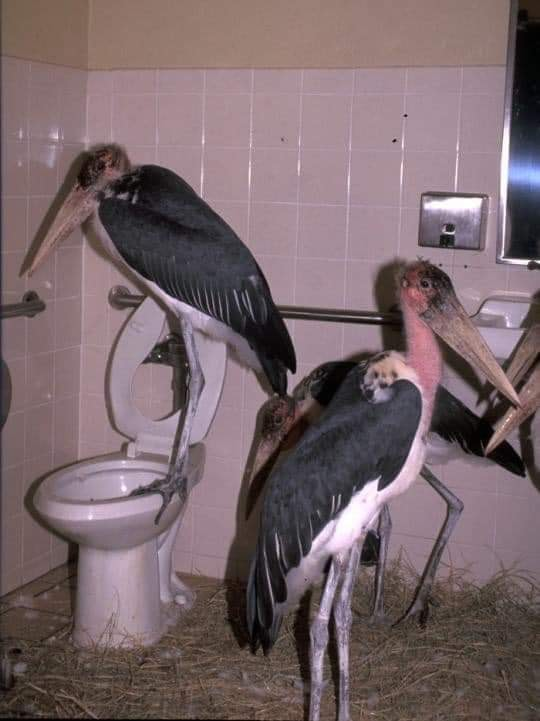
\includegraphics[height=100mm]{\frontpic}}} % the \FIG{} is optional
         {\ThesisYear}
  \TITLE{\theauthor}
        {\thesistitle}
\EndTitlePage
\titlepage\ \endtitlepage 

% Initial thesis pages
\TitlePage
  \HEADER{}{\ThesisYear}
  \TITLE{\theauthor{}}
        {\thesistitle}
  \vspace*{15mm}
  \TEXT{}
       {\thedeclaration}
\EndTitlePage
\titlepage\ \endtitlepage % empty page

\TitlePage
  \vspace*{55mm}
  \TEXT{\textbf{o j\'uri~/~the jury\newline}}
       {}
  \TEXT{presidente~/~president}
       {\textbf{\president}\newline {\small
        \presidentd \space (por delega\c c\~ao da Reitora da
        Universidade de Aveiro)}}
  \vspace*{5mm}
  \TEXT{vogais~/~examiners committee}
       {\textbf{\orientador}\newline {\small
        \orientadord \space (orientador)}}
  \vspace*{5mm}
  \TEXT{}
       {\textbf{\coorientador}\newline {\small
        \coorientadord \space (co-orientador)}}
  \vspace*{5mm}
  \TEXT{}
       {\textbf{\vogal}\newline {\small
        \vogald}}
\EndTitlePage
\titlepage\ \endtitlepage % empty page

\TitlePage
  \vspace*{55mm}
  \TEXT{\textbf{agradecimentos~/\newline acknowledgements}}
       {\'E com muito gosto que aproveito esta oportunidade para agradecer a todos os que me
        ajudaram durante este longos e penosos anos, cheios de altos e baixos (mais baixos que
        altos)\ldots}
  \TEXT{}
       {Desejo tamb\'em pedir desculpa a todos que tiveram de suportar o meu desinteresse pelas
        tarefas mundanas do dia-a-dia, \ldots}
\EndTitlePage
\titlepage\ \endtitlepage % empty page

\TitlePage
  \vspace*{55mm}
  \TEXT{\textbf{Resumo}}
       {Nos dias que correm, \'e frequente um trabalho ser avaliado pela sua apar\^encia em vez de
        o ser pelo seu conte\'udo. Sendo assim, sem descurar este \'ultimo, nesta tese descrevemos
        maneiras revolucion\'arias de transformar um documento s\'olido e austero num documento
        s\'olido e belo, capaz de fazer chorar de alegria (ou de inveja) qualquer leitor, mesmo
        quando este n\~ao percebe nada do que l\'a est\'a escrito.}
  \TEXT{}
       {A explora\c c\~ao de novas descobertas na \'area da percep\c c\~ao visual, nomeadamente
        no que se refere \`a aprecia\c c\~ao de obras de arte geniais, \ldots}
\EndTitlePage
\titlepage\ \endtitlepage % empty page

\TitlePage
  \vspace*{55mm}
  \TEXT{\textbf{Abstract}}
       {Nowadays, it is usual to evaluate a work \ldots}
\EndTitlePage
\titlepage\ \endtitlepage % empty page

% Tables of contents, of figures, ...

\pagenumbering{roman}
\tableofcontents

\cleardoublepage
\listoffigures

\cleardoublepage
\listoftables

% The chapters (usually written using the isolatin font encoding ...)

\cleardoublepage
\pagenumbering{arabic}

% Import here your chapters
\chapter{Introduction}

\section{Motivation: stocks control in warehouses in mall shops and in schools (space, different operators, number of operations)}

\section{Dissertation organization (to do later)}

%\section{Context}

Nespresso is owned by Nestlé Nespresso S. A., one operational 
unit of the Nestlé Group, with headquarters in Lausanne, 
Switzerland~\cite{nespressowebsite}. (...)

The proposed solution is a system around \textbf{smart shelving}. 

The structure storing the products contains RFID antennas and 
readers that detect and read the tags attach to them. Those 
readers will let the platform know in real time the state of 
the product in stock.

This system should handle the registration and verification 
of arriving stock and manage in real time warehouse products. 

The product should integrate with the logistics management 
software used by the company, allowing the a real-time 
management off all the products, machine learning predictions 
and control of the product flow.

The solution must be reliable and cheap to maintain. The 
initial investment should also be the smallest possible. 

%\section{Motivation}

With the growing of the brand, the complexity in the logistics 
networks starts to compromise the management of the products 
down in the chain. 

The categorization and verification of new inventory, inspection 
of the arrived goods from the transportation company, returns, 
control and management of stocks, are all attended by manual 
labour. 
The manual labour is prone to errors, takes a lot of working 
time and interfacing with the management software isn't usually 
efficient.

%\section{Objectives}

\begin{itemize}
  \item \textbf{Prevent stock-outs:} get timely replenishment 
  and optimizes in-store sales and management. Logistics 
  companies deliver goods on time and according to delivery 
  requirements;
  \item \textbf{Reduce time and errors from manual labour:} 
  counts, identification, misplacement and lost or stolen items;
  \item \textbf{Help customers:} find and engage with the 
  products they want;
  \item \textbf{Control:} who removes or checks out valuable 
  items;
  \item \textbf{Automatic information and management of stock:} 
  the logistics lines automatically transmits and receives 
  stock information;
  \item \textbf{Smart physical storage:} automatic 
  identification of goods in the warehouse/shelves, 
  automatic matching of distribution requirements, improves 
  the efficiency of goods storage;
  \item \textbf{Acquisition technology:} After the goods enter 
  the collection area, the collection equipment automatically 
  identifies multiple items by collecting RFID tags, thereby 
  efficiently completing the goods in and out of the warehouse, 
  ensuring whether the physical and distribution requirements 
  are consistent, and improving the efficiency of goods 
  distribution;
  \item \textbf{Real-time:} master the distribution of all 
  goods in real time, accurately grasp the inventory situation, 
  optimize the reasonable inventory, and grasp the status and 
  changes of the warehouse environment in real time;
\end{itemize}

%\cleardoublepage
% - history
% - overview da architectura (tag, antena, leitor)
% - basics da física
% - tecnologias (LF, HF), seus protocolos e aplicações
% .
% - UHF rain RFID
% - Problems (codigo de barras inoperability, diferentes standards )
% - solution of EPC (who is it) 
% - architecture solution
% - Tags: coding schemes, types ...
% - Reader and LLRP
% - Filtering & collection and ALE 

\chapter{State of the art}

\section{Basic principles of RFID}

\todo[color=yellow,inline]{History of RFID}
\todo[color=yellow,inline]{Physical overview (Induction and RF)}
\todo[color=yellow,inline]{Tecnologies (LF, HF, UHF, Microwave)}
\todo[color=yellow,inline]{RFID System (tag, antenna, reader)}
\todo[color=yellow,inline]{Advantages and Limitations}
\todo[inline]{Toughts on the hurdles of RFID: to expensive, to complex, might not provide business advantages, no one has all the expertise, everyone is still learning}
\todo[color=yellow,inline]{Application Areas}

\section{UHF RFID Architecture}

\subsection{Global Standardization}

\subsubsection{Importance}

\todo[color=yellow,inline]{The importance of a end-to-end architecture standard (enables comunication between every member in the value chain)}

\subsubsection{Efforts}

Standardization of \gls{UHF RFID} for item level tagging and \gls{supply chain}, by organizations like \gls{GS1}, provided a common language to identify, capture and share supply chain data, ensuring important information is accessible, accurate and easy to understand~\cite{anonymousStandardsGS12014}.

The first prominent adoption was by the \gls{DoD} with a policy released on July 30th 2004. The policy stated that contracts issued for material delivery would require the use of RFID tags. The policy was later extended to all commodities and commodities pallets shipped to any \gls{DoD} facility~\cite{DoDSuppliersPassive, DODReleasesFinal}.

In 2014, Impinj, Intel, Google and Smartrac, joined forces to create the \gls{RAIN RFID} alliance~\cite{TechnologyCompaniesCreate} after the ratification of \gls{GS1}'s \gls{UHF RFID} Generation 2 version 2 standard in November of 2013. The alliance promotes the universal adoption of \gls{GS1}'s Gen2 \gls{UHF RFID} technologies and the connection with \gls{cloud computing}, where RFID-based data can be stored, managed and shared via the Internet~\cite{WhatRAINRFID}.
The alliance fortified the adoption of \gls{GS1}'s standards and traced a common path for the the industry to progress.

On October 11th 2018 the European Commission published their positive implementing of the upper band in Europe~\cite{302208v030101pPdf}.
It extended the power levels to $2W$ in the lower band and added the requested global band from $915$MHz to $921$MHz with power levels up to $4W$. 
This was the biggest effort by the European Commission to establish a global standardized frequency band for \gls{UHF RFID} \gls{supply chain} applications.

\subsubsection{Current Problems}

\todo[color=yellow,inline]{International Standardization in UHF band RFID: problems (conformity, different standards and codding schemes), EU UHF RFID Upper band (countries that don't want to adopt, same frequency has IoT devices)}

\subsection{GS1}

The GS1 is a nonprofit organization dedicated to the development and implementation of standards for global \gls{supply chain} solutions. 
The institution mission is to manage the GS1 System of Standards, create open, global, multi-sector standards fostering good business practices.

GS1 established itself in 2005 from the \gls{EAN} International, \gls{UCC} and other local organizations from the United States~\cite{PublicationLEBENSMITTELZEITUNGa}.
The organization took under its umbrella the former EAN-UCC roles subsuming their technologies. From those, worth mentioning: the barcode identification system (from \gls{EAN}), \gls{XML} standards, \gls{EDI} transaction sets and \gls{supply chain} solutions~\cite[p.~212]{lahiriRFIDSourcebook2005}.

The new GS1 organization then adopted much more ambitious projects, developing global standards and services for business communication.
From those efforts resulted the network for the synchronization of master data \gls{GDSN}, the \gls{EPC} integration for \gls{RFID}, traceability and the upstream integration of the consumer goods industry suppliers and EPCglobal Network.

\section{EPCglobal Architecture Framework}

EPCglobal Architecture Framework is a collection of interrelated hardware, software, and data standards (\emph{EPCglobal Standards}) that interoperate with shared network services (\emph{EPC Network Services}) operated by GS1, its delegates, and others~\cite{Architecture6framework20140414Pdf}.

The existence of this standards promotes not only the global adoption of \gls{EPC}, but also the exchange of information between business partners. This frees the market of \emph{information systems} to create custom business solutions, since the standards only define the interfaces.

The architecture establishes three core requirements and activities, all of which have a group of standards within the \emph{EPCglobal Architecture Framework}.

\paragraph{Physical Object Exchange} 

\emph{Identify} individual products, cases, loads, assets, return items, among others, so they can be tracked individually.
The \emph{End Users} are parties in a supply chain that exchange physical objects that are identified with \gls{EPC}.
Physical object exchange consists in operations such as shipping, receiving goods, and so on.
For many End Users, the physical objects are trade goods, but this could not be the case.
There are many other uses, like library or asset management applications~\cite{dong-yingliDesignInternetThings2016} that differ from the \gls{supply chain} trade goods model, but still involve the requirement for unique identification and tagging of objects. 
The architecture must be designed to ensure that when one end user delivers a physical object to another end user, the latter will be able to determine the \gls{EPC} of the physical object and interpret it properly~\cite{Architecture6framework20140414Pdf}.
The \emph{EPCglobal Architecture Framework} defines \gls{EPC} physical object exchange standards.

\paragraph{Infrastructure for Data Capture} 

\emph{Capture data} about the movement of physical assets and creating visibility.
In order to have gather \gls{EPC} data, each \emph{End User} carries out operations within its environment. That can be the creation of \gls{EPC}s for new objects, follow the movements of objects by sensing their \gls{EPC}s, and gather that information into systems of record within the organization~\cite{Architecture6framework20140414Pdf}. The \emph{EPCglobal Architecture Framework} defines interface standards for the major infrastructure components required to gather and record \gls{EPC} data. This allows \emph{End Users} to develop their internal systems using interoperable components.

\paragraph{Data Sharing} 

\emph{Exchange data} with \gls{IT} applications and trading partners, to turn visibility into information and action.
\emph{End Users} benefit from the \emph{EPCglobal Architecture Framework} by sharing data with each other, increasing the visibility they have with respect to the movement of physical objects through the \gls{supply chain}. 
The \emph{EPCglobal Architecture Framework} defines \gls{EPC} data sharing standards, which provide a means for end users to share data about \gls{EPC}s within defined user groups or with the general public, and which also provide access to \emph{EPC Network Services} and other shared services that facilitate this sharing. \todo{change phrasing a bit}

\begin{figure}[!ht]
    \centering
    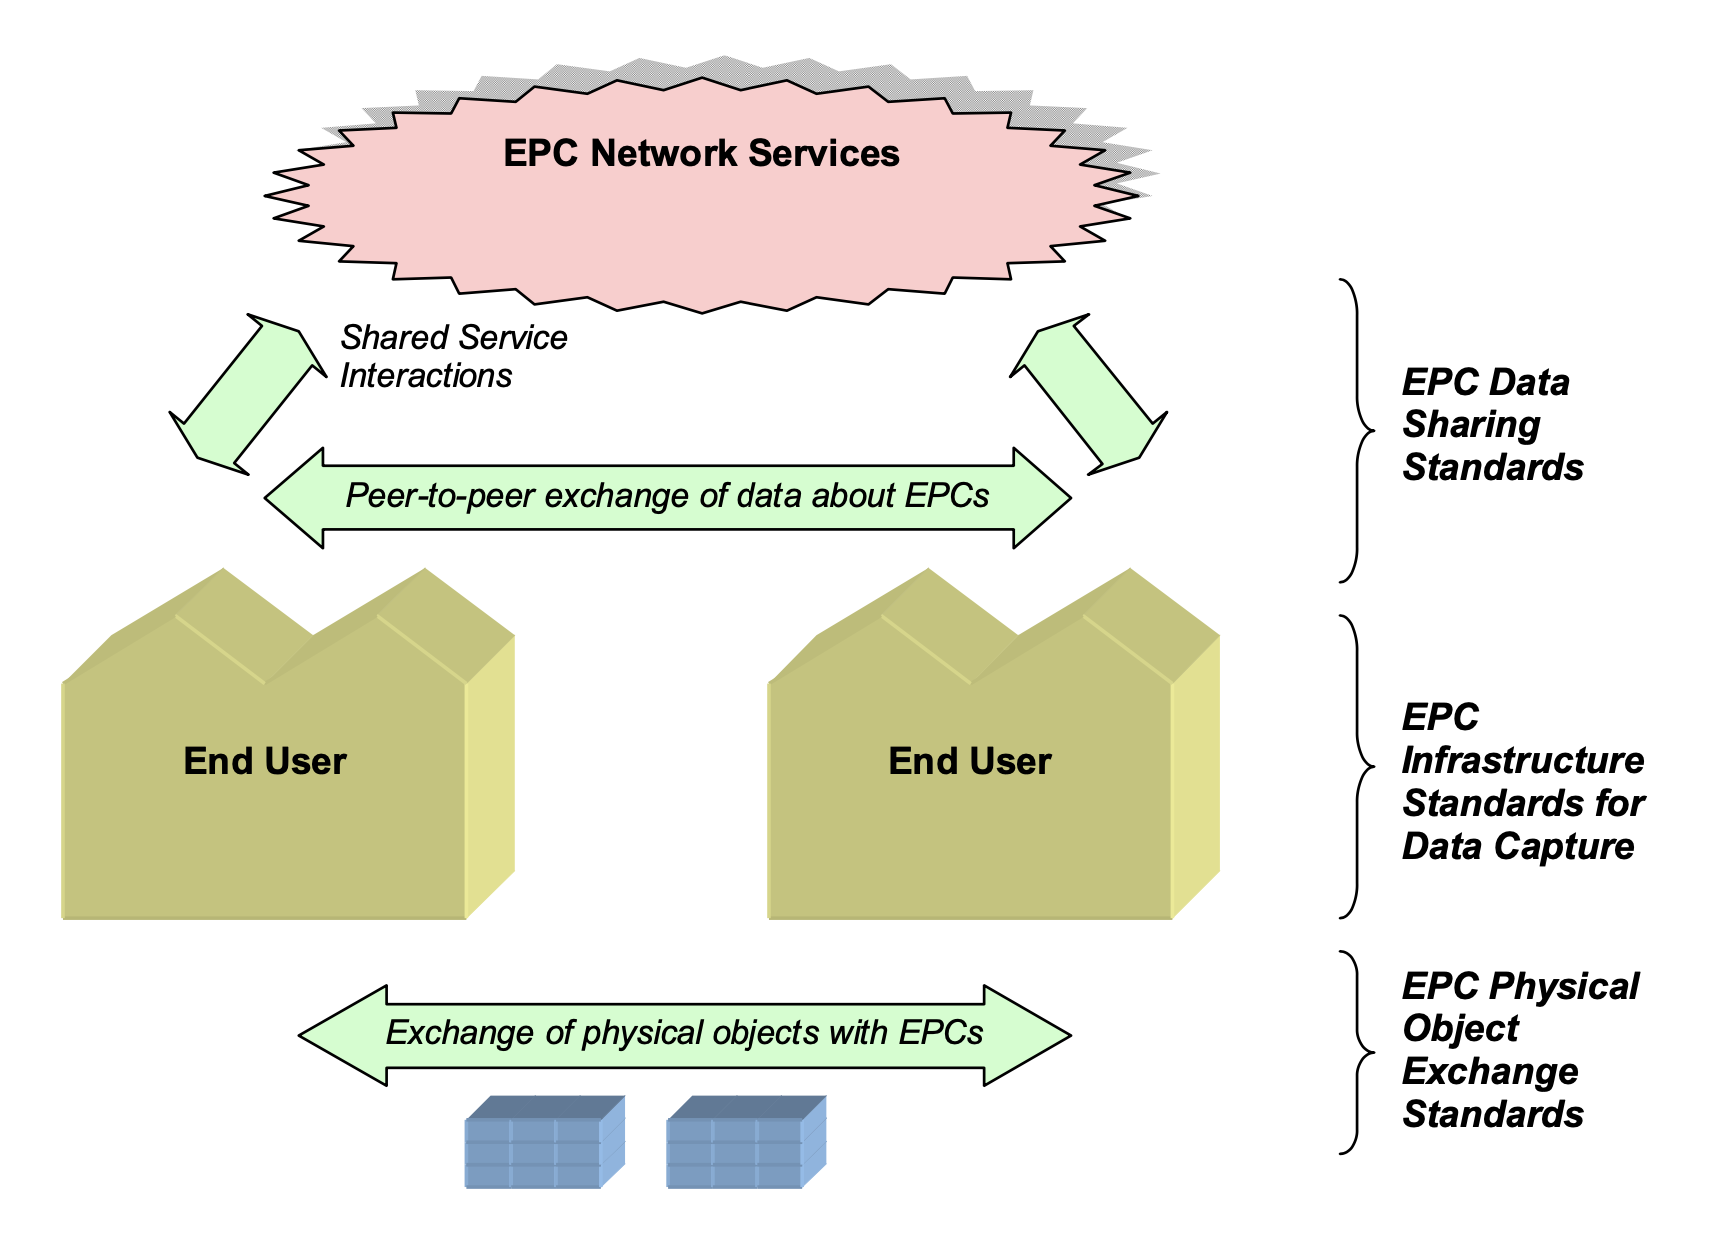
\includegraphics[width=0.9\textwidth]{./assets/02-state-of-the-art/architecture-framework-activities.png}
    \caption{\emph{EPCglobal Architecture Framework} activities~\cite{Architecture6framework20140414Pdf}} 
    \label{fig:02:architecture-activities}
\end{figure}

\subsection{EPCglobal Specification}

For RFID Technology to become viable in practice, an infrastructure must exist for processing and communicating EPC data. In meeting the goal of creating a common infrastructure, MIT announced Auto-ID Release 1.0 in October 2003. At the same time, MIT entered into an exclusive licensing agreement with GS1.
In turn, GS1 established a new division called EPCglobal to implement Release 1.0 and to conduct further development based on industry input. This put forth an initial set of standards that formed the basis of an infra- structure for EPC data. Later, Auto-ID Release 1.0 became the starting-point for the EPCglobal Network~\cite[p. 50]{GlobalRFIDValue}. \todo[color=red]{Rewrite this}

\todo[color=yellow,inline]{EPCglobal Spec history and context}

\subsection{EPCglobal Network}

The \emph{EPCglobal Network} is a computer network used to share \gls{EPC} data between trading partners. 
It provides automatic, real-time identification and data sharing of items both within and outside of an company~\cite[p. 213]{lahiriRFIDSourcebook2005}.

Even doe the network was design mainly for \gls{RFID} sharing of \gls{EPC} data, the network does not exclusively runs on \gls{RFID} data carriers. The \emph{EPCglobal Network} can also be fed \gls{EPC} data through data carriers like 1D and 2D barcodes. The interoperability with the barcode was one of the most important considerations used during the planning of the network~\cite{RFIDBarcodeInteroperability}.

\todo[color=yellow,inline]{GS1 Architecture: organization, advantages and objectives: barcode inoperability}

\subsection{EPC}

The basis for the information flow in the network is the Electronic Product Code (EPC), which is a universally unique identifier for any physical object anywhere in the world, for all time. 
The EPC may be encoded in a Radio Frequency Identification (RFID) tag but is not designed exclusively for use with RFID data carriers. For example, EPCs can also be constructed based on the reading of optical data carriers, such as linear barcodes.

\todo[color=yellow,inline]{Classes, codding schemes: 1 Gen 2 or ISO/IEC18000-6 Type C: ISO adoption of GS1's C1G2}

\subsubsection{EPC in EPCglobal Architecture Framework}

\todo[inline]{Check page 24 of the GS1 EPCglobal architecture Framework pdf}


\subsection{Data-Collection}

\subsubsection{Hardware}

\subsubsection{Low Level Reader Protocol (LLRP)}

\subsection{Middleware}

\subsubsection{Application Level Events (ALE)}

\subsection{\gls{EPC} Information Services (EPCIS)}

\subsection{Discovery Services}

\subsection{All working together}

\todo[color=yellow,inline]{All working together (brief on the everything working together)}

\section{Overview of the overall solutions}

\subsection{Commercial solutions}

\todo[color=yellow,inline]{Analisys of commercial antenna/reader solutions}

\subsection{Academic solutions}

\todo[inline]{Work of Andrea D’Alessandro~\cite{dalessandroRFIDBasedSmartShelving2012}}
\todo[inline]{Robots for warehouse scan}
%\chapter{Requirements and Development Options}

\section{System requirements: shelves for Nespresso, lockers, shelves for schools}

\section{Manufacturers and development solutions: comparative analysis}

\section{Out choice: justification; a bit of detail}

%\chapter{System Architecture and development}

\section{Overall architecture}

\section{Specific solutions (detection)}

\subsection{Nespresso}

\subsection{Lockers}

\subsection{Schools}

\section{Embedded system architecture}

\section{Software solutions for reading and localization}

\section{Communication and web platform}
%\chapter{Test and evaluation}

\section{Laboratory tests: put and take}

\section{Range of operation tests (to verify if it reads the number of items stored; RSSIs and other technical operational values, stress tests)}

\section{Operational tests (real case)}
%\chapter{Conclusion and Future Work}

\section{Retell the story from motivation to results}

\section{Main achievements}

\section{Future Work - worth hadn't time to do but must be done}

% Back cover, bibliography and attachments
\bibliographystyle{unsrt}
\bibliography{biblio.bib}
%\cleardoublepage

\end{document}
